% !TeX program = xelatex
\documentclass{article}
\usepackage{kotex}
\usepackage[a4paper,left=3cm, right=3cm, top=2cm, bottom=2cm]{geometry}
\usepackage{amsmath}
\usepackage{graphicx}
\usepackage{caption}
\usepackage{setspace}
\usepackage{xcolor}
\usepackage{titlesec}
\usepackage{amssymb}
\usepackage{tcolorbox}
\usepackage{amsthm}
\usepackage{multirow}
\usepackage{array}
\usepackage{booktabs}
\usepackage{tikz}
\usetikzlibrary{positioning,arrows.meta,calc,matrix,decorations.pathreplacing}
\usepackage{cancel}
\usepackage{pgfplots}
\pgfplotsset{compat=1.18}

\title{9.4 Singular Value Decomposition}
\date{}
\author{}
\setstretch{1.3}

\titleformat{name=\section, numberless}
  {\normalfont\large\bfseries\color{blue}}{}
  {0pt}{}
\geometry{a4paper, margin=1in}

\newcommand{\redheading}[1]{{\vspace{2mm}\noindent\Large\bfseries\color{red!55!black} #1\par}\vspace{2mm}}

\begin{document}
\maketitle

{\itshape\color{blue!45!black}
In this section we discuss an extension of the diagonalization theory for $n\times n$
symmetric matrices to general $m\times n$ matrices. The results have applications to
compression, storage, and transmission of digitized information and form the basis for
many of the best computational algorithms currently available for solving linear
systems.\par}

\vspace{2mm}

\redheading{Decompositions of Square Matrices}

Recall from Section~7.2 that every symmetric matrix $A$ with real entries has an
\textbf{eigenvalue decomposition}
\[
  A = PDP^T \tag{1}
\]
where $P$ is orthogonal (columns are eigenvectors of $A$) and $D$ is diagonal
(eigenvalues of $A$). For non-symmetric $n\times n$ matrices, two further
decompositions exist:
\begin{itemize}
  \item \textbf{Hessenberg decomposition} (Theorem~7.2.4): $A = PHP^T$ ($P$ orthogonal,
        $H$ upper Hessenberg).
  \item \textbf{Schur decomposition} (Theorem~7.2.3, when $A$ has real eigenvalues):
        $A = PSP^T$ ($P$ orthogonal, $S$ upper triangular).
\end{itemize}
These are important numerically because orthogonal matrices do not magnify roundoff
error ($\|P\mathbf{x} - P\hat{\mathbf{x}}\| = \|\mathbf{x}-\hat{\mathbf{x}}\|$).

For a general $m\times n$ matrix $A$, the factorization of the form
\[
  A = U\Sigma V^T
\]
where $U$ and $V$ are orthogonal (but generally different) is called the
\textbf{singular value decomposition} (SVD) of $A$.

\vspace{2mm}
\redheading{Singular Values}

Since matrix products of the form $A^TA$ play a central role, we start with two theorems.

\begin{tcolorbox}[colback=red!4, colframe=red!60!black,
  title={\textbf{Theorem 9.4.1}}, boxrule=0.5mm, arc=3mm]
If $A$ is an $m\times n$ matrix, then:
\begin{itemize}
  \item[(a)] $A$ and $A^TA$ have the same null space.
  \item[(b)] $A$ and $A^TA$ have the same row space.
  \item[(c)] $A^T$ and $A^TA$ have the same column space.
  \item[(d)] $A$ and $A^TA$ have the same rank.
\end{itemize}
\end{tcolorbox}

\textit{Proof of (a).} We show every solution of $A\mathbf{x}=\mathbf{0}$ is also a
solution of $A^TA\mathbf{x}=\mathbf{0}$, and vice versa. If $A\mathbf{x}_0=\mathbf{0}$,
then $A^TA\mathbf{x}_0 = A^T(A\mathbf{x}_0) = A^T\mathbf{0} = \mathbf{0}$. Conversely,
if $A^TA\mathbf{x}_0=\mathbf{0}$, then $\mathbf{x}_0$ is orthogonal to every vector in
$\mathrm{col}(A^TA) = \mathrm{col}(A^T)$ (the row space of $A$), so $\mathbf{x}_0$ is
in the null space of $A$. Alternatively:
\[
  \mathbf{x}_0^T(A^TA)\mathbf{x}_0 = (A\mathbf{x}_0)^T(A\mathbf{x}_0)
  = \|A\mathbf{x}_0\|^2 = 0 \implies A\mathbf{x}_0 = \mathbf{0}.\quad\blacksquare
\]

\begin{tcolorbox}[colback=red!4, colframe=red!60!black,
  title={\textbf{Theorem 9.4.2}}, boxrule=0.5mm, arc=3mm]
If $A$ is an $m\times n$ matrix, then:
\begin{itemize}
  \item[(a)] $A^TA$ is orthogonally diagonalizable.
  \item[(b)] The eigenvalues of $A^TA$ are nonneg\-ative real numbers.
\end{itemize}
\end{tcolorbox}

\textit{Proof.} (a) $A^TA$ is symmetric, so Theorem~7.2.1 applies. (b) Let
$\{\mathbf{v}_1,\ldots,\mathbf{v}_n\}$ be an orthonormal eigenbasis for $A^TA$ with
eigenvalues $\lambda_1,\ldots,\lambda_n$. For $1\le i\le n$:
\[
  \|A\mathbf{v}_i\|^2 = A\mathbf{v}_i\cdot A\mathbf{v}_i
  = \mathbf{v}_i\cdot A^TA\mathbf{v}_i
  = \mathbf{v}_i\cdot\lambda_i\mathbf{v}_i = \lambda_i\|\mathbf{v}_i\|^2 = \lambda_i \ge 0.
  \quad\blacksquare
\]

We assume throughout that the eigenvalues of $A^TA$ are ordered so that
$\lambda_1\ge\lambda_2\ge\cdots\ge\lambda_n\ge 0$.

\begin{tcolorbox}[colback=teal!4, colframe=teal!65!black,
  title={\textbf{Definition 1}}, boxrule=0.5mm, arc=3mm]
If $A$ is an $m\times n$ matrix with eigenvalues $\lambda_1,\lambda_2,\ldots,\lambda_n$
of $A^TA$ (in nonincreasing order), then the numbers
\[
  \sigma_1 = \sqrt{\lambda_1},\quad \sigma_2 = \sqrt{\lambda_2},\quad\ldots,\quad
  \sigma_n = \sqrt{\lambda_n}
\]
are called the \textbf{singular values} of $A$.
\end{tcolorbox}

\subsection*{EXAMPLE 1 | Singular Values}

Find the singular values of $A = \begin{bmatrix}1&1\\0&1\\1&0\end{bmatrix}$.

\textbf{SOLUTION:}
\[
  A^TA = \begin{bmatrix}1&0&1\\1&1&0\end{bmatrix}
         \begin{bmatrix}1&1\\0&1\\1&0\end{bmatrix}
       = \begin{bmatrix}2&1\\1&2\end{bmatrix}
\]
Characteristic polynomial: $\lambda^2 - 4\lambda + 3 = (\lambda-3)(\lambda-1) = 0$,
so $\lambda_1=3,\ \lambda_2=1$. The singular values of $A$ are
\[
  \sigma_1 = \sqrt{3},\qquad \sigma_2 = 1.
\]

\vspace{2mm}
\redheading{Singular Value Decomposition}

The \textbf{main diagonal} of an $m\times n$ matrix is the sequence of entries
$a_{11},a_{22},\ldots$ as far as the matrix extends diagonally
(see Figure~9.4.1). Entries on the main diagonal are called \textbf{diagonal entries}.

\begin{figure}[ht]
\centering
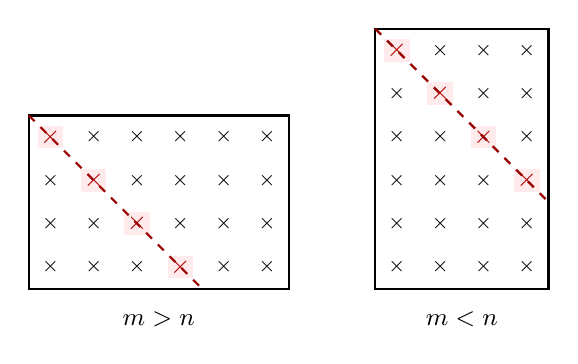
\begin{tikzpicture}[scale=0.55]
  \draw[thick] (0,0) rectangle (6,4);
  \foreach \i in {0,1,2,3} {
    \foreach \j in {0,1,2,3,4,5} {
      \node[font=\scriptsize] at (0.5+\j, 3.5-\i) {$\times$};
    }
  }
  \foreach \i in {0,1,2,3} {
    \node[font=\small, red!70!black, fill=red!8, inner sep=1pt]
      at (0.5+\i, 3.5-\i) {$\times$};
  }
  \draw[red!60!black, thick, dashed] (0,4) -- (4,0);
  \node[below, font=\small] at (3,-0.3) {$m>n$};
  \begin{scope}[xshift=8cm]
    \draw[thick] (0,0) rectangle (4,6);
    \foreach \i in {0,1,2,3,4,5} {
      \foreach \j in {0,1,2,3} {
        \node[font=\scriptsize] at (0.5+\j, 5.5-\i) {$\times$};
      }
    }
    \foreach \i in {0,1,2,3} {
      \node[font=\small, red!70!black, fill=red!8, inner sep=1pt]
        at (0.5+\i, 5.5-\i) {$\times$};
    }
    \draw[red!60!black, thick, dashed] (0,6) -- (4,2);
    \node[below, font=\small] at (2,-0.3) {$m<n$};
  \end{scope}
\end{tikzpicture}
\caption*{FIGURE 9.4.1\quad Main diagonals of non-square matrices}
\end{figure}

\begin{tcolorbox}[colback=red!4, colframe=red!60!black,
  title={\textbf{Theorem 9.4.3 --- Singular Value Decomposition (Brief Form)}},
  boxrule=0.5mm, arc=3mm]
If $A$ is an $m\times n$ matrix of rank $k$, then $A$ can be expressed as
$A = U\Sigma V^T$, where $\Sigma$ has size $m\times n$ and partitioned form
\[
  \Sigma = \left[\begin{array}{c|c}
    D & \mathbf{0}_{k\times(n-k)}\\
    \hline
    \mathbf{0}_{(m-k)\times k} & \mathbf{0}_{(m-k)\times(n-k)}
  \end{array}\right]
\]
$D = \mathrm{diag}(\sigma_1,\sigma_2,\ldots,\sigma_k)$ contains the nonzero singular
values in nonincreasing order, $U$ is an $m\times m$ orthogonal matrix, and $V$ is an
$n\times n$ orthogonal matrix.
\end{tcolorbox}

\begin{tcolorbox}[colback=red!4, colframe=red!60!black,
  title={\textbf{Theorem 9.4.4 --- Singular Value Decomposition (Expanded Form)}},
  boxrule=0.5mm, arc=3mm]
If $A$ is an $m\times n$ matrix of rank $k$, then $A$ can be factored as
\[
  A = U\Sigma V^T = [\mathbf{u}_1\ \mathbf{u}_2\ \cdots\ \mathbf{u}_k\ |\ \mathbf{u}_{k+1}\ \cdots\ \mathbf{u}_m]
  \begin{bmatrix}
    \sigma_1 & & & & \mathbf{0}\\
    & \sigma_2 & & &\\
    & & \ddots & &\\
    & & & \sigma_k &\\
    \hline
    \multicolumn{4}{c}{\mathbf{0}} & \mathbf{0}
  \end{bmatrix}
  \begin{bmatrix}\mathbf{v}_1^T\\\mathbf{v}_2^T\\\vdots\\\mathbf{v}_k^T\\\mathbf{v}_{k+1}^T\\\vdots\\\mathbf{v}_n^T\end{bmatrix}
\]
in which $U$, $\Sigma$, $V$ have sizes $m\times m$, $m\times n$, $n\times n$, and:
\begin{itemize}
  \item[(a)] $V = [\mathbf{v}_1\ \mathbf{v}_2\ \cdots\ \mathbf{v}_n]$ orthogonally diagonalizes $A^TA$.
  \item[(b)] Nonzero diagonal entries of $\Sigma$ are $\sigma_i = \sqrt{\lambda_i}$,
        where $\lambda_1,\ldots,\lambda_k$ are the nonzero eigenvalues of $A^TA$
        corresponding to column vectors of $V$.
  \item[(c)] Columns of $V$ are ordered so $\sigma_1\ge\sigma_2\ge\cdots\ge\sigma_k>0$.
  \item[(d)] $\mathbf{u}_i = \dfrac{A\mathbf{v}_i}{\|A\mathbf{v}_i\|} = \dfrac{1}{\sigma_i}A\mathbf{v}_i$
        \quad$(i=1,2,\ldots,k)$.
  \item[(e)] $\{\mathbf{u}_1,\mathbf{u}_2,\ldots,\mathbf{u}_k\}$ is an orthonormal basis for $\mathrm{col}(A)$.
  \item[(f)] $\{\mathbf{u}_1,\ldots,\mathbf{u}_k,\mathbf{u}_{k+1},\ldots,\mathbf{u}_m\}$ is an
        orthonormal basis for $R^m$.
\end{itemize}
The vectors $\mathbf{u}_1,\ldots,\mathbf{u}_k$ are \textbf{left singular vectors} and
$\mathbf{v}_1,\ldots,\mathbf{v}_k$ are \textbf{right singular vectors} of $A$.
\end{tcolorbox}

\textit{Proof.}
We prove the theorem for the case where $A$ is $n\times n$; the rectangular case requires
only notational adjustments.

\textbf{Step 1: Orthonormal eigenbasis for $A^TA$.}
By Theorem~9.4.2(a), $A^TA$ is orthogonally diagonalizable. Let
$\{\mathbf{v}_1,\ldots,\mathbf{v}_n\}$ be an orthonormal eigenbasis for $R^n$ with
eigenvalues $\lambda_1\ge\lambda_2\ge\cdots\ge\lambda_n\ge 0$. Since $\mathrm{rank}(A)=k$,
Theorem~9.4.1(d) gives $\mathrm{rank}(A^TA)=k$, so exactly $k$ eigenvalues are positive:
$\lambda_1\ge\cdots\ge\lambda_k>0$ and $\lambda_{k+1}=\cdots=\lambda_n=0$.

\textbf{Step 2: $\{A\mathbf{v}_1,\ldots,A\mathbf{v}_k\}$ is an orthogonal set of nonzero
vectors.}
For $1\le i\le k$:
\[
  \|A\mathbf{v}_i\|^2 = \mathbf{v}_i\cdot A^TA\mathbf{v}_i
  = \mathbf{v}_i\cdot\lambda_i\mathbf{v}_i = \lambda_i\|\mathbf{v}_i\|^2 = \lambda_i > 0
\]
so each $A\mathbf{v}_i\ne\mathbf{0}$. For $i\ne j$ (both $\le k$):
\[
  A\mathbf{v}_i\cdot A\mathbf{v}_j = \mathbf{v}_i\cdot A^TA\mathbf{v}_j
  = \mathbf{v}_i\cdot\lambda_j\mathbf{v}_j = \lambda_j(\mathbf{v}_i\cdot\mathbf{v}_j) = 0
\]
since $\{\mathbf{v}_i\}$ is orthonormal. For $i>k$: $\|A\mathbf{v}_i\|^2=\lambda_i=0$,
so $A\mathbf{v}_i=\mathbf{0}$.

\textbf{Step 3: $S=\{A\mathbf{v}_1,\ldots,A\mathbf{v}_k\}$ is an orthogonal basis for
$\mathrm{col}(A)$.}
$S$ consists of $k$ nonzero orthogonal vectors, hence linearly independent. Since each
$A\mathbf{v}_i\in\mathrm{col}(A)$ and $\dim\mathrm{col}(A)=k$, $S$ is a basis for
$\mathrm{col}(A)$.

\textbf{Step 4: Left singular vectors (part (d)) and orthonormal basis for $\mathrm{col}(A)$
(part (e)).}
Define
\[
  \mathbf{u}_i = \frac{A\mathbf{v}_i}{\|A\mathbf{v}_i\|} = \frac{1}{\sqrt{\lambda_i}}A\mathbf{v}_i
  = \frac{1}{\sigma_i}A\mathbf{v}_i \qquad (i=1,2,\ldots,k)
\]
Normalizing the orthogonal basis $S$ gives the orthonormal set
$\{\mathbf{u}_1,\ldots,\mathbf{u}_k\}$, which is therefore an orthonormal basis for
$\mathrm{col}(A)$. Equivalently,
\begin{equation}
  A\mathbf{v}_i = \sigma_i\mathbf{u}_i \qquad (i=1,\ldots,k) \tag{4}
\end{equation}

\textbf{Step 5: Orthonormal basis for $R^m$ (part (f)).}
By the Gram--Schmidt process (Theorem~6.3.6), extend
$\{\mathbf{u}_1,\ldots,\mathbf{u}_k\}$ to an orthonormal basis
$\{\mathbf{u}_1,\ldots,\mathbf{u}_k,\mathbf{u}_{k+1},\ldots,\mathbf{u}_m\}$ for $R^m$.
Let $U = [\mathbf{u}_1\ \cdots\ \mathbf{u}_m]$ (orthogonal, $m\times m$) and
$V = [\mathbf{v}_1\ \cdots\ \mathbf{v}_n]$ (orthogonal, $n\times n$).

\textbf{Step 6: $A = U\Sigma V^T$.}
It suffices to show $AV = U\Sigma$, since $V^{-1}=V^T$ then gives $A = U\Sigma V^T$.
Compare column $i$ of each side:
\begin{itemize}
  \item For $i\le k$: column $i$ of $AV$ is $A\mathbf{v}_i = \sigma_i\mathbf{u}_i$
        (by~(4)), and column $i$ of $U\Sigma$ is $\sigma_i\mathbf{u}_i$ (the $i$th
        column of $\Sigma$ has $\sigma_i$ in row $i$ and zeros elsewhere, so
        $U\Sigma\mathbf{e}_i = \sigma_i\mathbf{u}_i$). \checkmark
  \item For $i>k$: column $i$ of $AV$ is $A\mathbf{v}_i = \mathbf{0}$ (Step~2), and
        column $i$ of $U\Sigma$ is $\mathbf{0}$ (the $i$th column of $\Sigma$ is all
        zeros). \checkmark
\end{itemize}
Hence $AV = U\Sigma$, and multiplying on the right by $V^T$ gives $A = U\Sigma V^T$.
$\blacksquare$

\subsection*{EXAMPLE 2 | Singular Value Decomposition (Non-Square $A$)}

Find a singular value decomposition of $A = \begin{bmatrix}1&1\\0&1\\1&0\end{bmatrix}$.

\textbf{SOLUTION:} From Example~1, $\lambda_1=3,\ \lambda_2=1$ and $\sigma_1=\sqrt{3},\
\sigma_2=1$. One can verify that
\[
  \mathbf{v}_1 = \begin{bmatrix}\tfrac{\sqrt{2}}{2}\\\tfrac{\sqrt{2}}{2}\end{bmatrix},\qquad
  \mathbf{v}_2 = \begin{bmatrix}\tfrac{\sqrt{2}}{2}\\-\tfrac{\sqrt{2}}{2}\end{bmatrix}
\]
are eigenvectors of $A^TA$ corresponding to $\lambda_1=3$ and $\lambda_2=1$, so
$V = [\mathbf{v}_1\mid\mathbf{v}_2]$ orthogonally diagonalizes $A^TA$.

From Theorem~9.4.4(d):
\[
  \mathbf{u}_1 = \frac{1}{\sqrt{3}}A\mathbf{v}_1
  = \frac{\sqrt{3}}{3}\begin{bmatrix}1&1\\0&1\\1&0\end{bmatrix}
    \begin{bmatrix}\tfrac{\sqrt{2}}{2}\\\tfrac{\sqrt{2}}{2}\end{bmatrix}
  = \begin{bmatrix}\tfrac{\sqrt{6}}{3}\\\tfrac{\sqrt{6}}{6}\\\tfrac{\sqrt{6}}{6}\end{bmatrix},
  \qquad
  \mathbf{u}_2 = \frac{1}{1}A\mathbf{v}_2 = \begin{bmatrix}0\\-\tfrac{\sqrt{2}}{2}\\\tfrac{\sqrt{2}}{2}\end{bmatrix}
\]
To find $\mathbf{u}_3$, we need a unit vector orthogonal to both $\sqrt{6}\,\mathbf{u}_1 = (2,1,1)^T$
and $\sqrt{2}\,\mathbf{u}_2 = (0,-1,1)^T$. Solving the homogeneous system gives
general solution $t(-1,1,1)^T$, so normalizing:
\[
  \mathbf{u}_3 = \begin{bmatrix}-\tfrac{1}{\sqrt{3}}\\\tfrac{1}{\sqrt{3}}\\\tfrac{1}{\sqrt{3}}\end{bmatrix}
\]
Thus the SVD of $A$ is
\[
  \begin{bmatrix}1&1\\0&1\\1&0\end{bmatrix}
  = \underbrace{\begin{bmatrix}
      \tfrac{\sqrt{6}}{3} & 0 & -\tfrac{1}{\sqrt{3}}\\
      \tfrac{\sqrt{6}}{6} & -\tfrac{\sqrt{2}}{2} & \tfrac{1}{\sqrt{3}}\\
      \tfrac{\sqrt{6}}{6} & \tfrac{\sqrt{2}}{2} & \tfrac{1}{\sqrt{3}}
    \end{bmatrix}}_{U}
  \underbrace{\begin{bmatrix}\sqrt{3}&0\\0&1\\0&0\end{bmatrix}}_{\Sigma}
  \underbrace{\begin{bmatrix}
      \tfrac{\sqrt{2}}{2} & \tfrac{\sqrt{2}}{2}\\
      \tfrac{\sqrt{2}}{2} & -\tfrac{\sqrt{2}}{2}
    \end{bmatrix}}_{V^T}
\]

\vspace{3mm}
\noindent\rule{\linewidth}{0.5pt}

\section*{Exercise Set 9.4}

\noindent\textit{In Exercises 1--4, find the distinct singular values of $A$.}

\begin{enumerate}
  \item $A = \begin{bmatrix}1&2&0\end{bmatrix}$

  \item $A = \begin{bmatrix}3&0\\0&4\end{bmatrix}$

  \item $A = \begin{bmatrix}1&-2\\2&1\end{bmatrix}$

  \item $A = \begin{bmatrix}\sqrt{2}&0\\1&\sqrt{2}\end{bmatrix}$

\end{enumerate}

\noindent\textit{In Exercises 5--8, find a singular value decomposition of $A$.}

\begin{enumerate}
  \item[5.] $A = \begin{bmatrix}1&-1\\1&1\end{bmatrix}$

  \item[6.] $A = \begin{bmatrix}-3&0\\0&-4\end{bmatrix}$

  \item[7.] $A = \begin{bmatrix}4&6\\0&4\end{bmatrix}$

  \item[9.] $A = \begin{bmatrix}-2&2\\-1&1\\2&-2\end{bmatrix}$

\end{enumerate}

\noindent\textit{Working with Proofs}

\begin{enumerate}
  \item[13.] Prove: If $A$ is an $m\times n$ matrix, then $A$ and $A^TA$ have the same
        rank.

  \item[14.] Prove part (d) of Theorem~9.4.1 by using part (a) and the fact that $A$
        and $A^TA$ have $n$ columns.

  \item[17.] Prove that the singular values of $A^TA$ are the squares of the singular
        values of $A$.

  \item[18.] Prove: If $A = U\Sigma V^T$ is a singular value decomposition of $A$, then
        $U$ orthogonally diagonalizes $AA^T$.

  \item[19.] A \textbf{polar decomposition} of an $n\times n$ matrix $A$ is a
        factorization $A = PQ$ where $P$ is positive semidefinite with the same rank
        as $A$, and $Q$ is orthogonal.

        \textbf{a.} Prove: If $A = U\Sigma V^T$ is a singular value decomposition of $A$,
        then $A = (U\Sigma U^T)(UV^T)$ is a polar decomposition of $A$.

        \textbf{b.} Find a polar decomposition of the matrix in Exercise~5.

\end{enumerate}

\end{document}
